\documentclass{article}

\usepackage{minitoc}
\usepackage{tabularx}
\usepackage{booktabs}
\usepackage{graphicx}
\usepackage{hyperref}
\usepackage{xcolor}
\usepackage{blkarray}
\usepackage{amsthm, amssymb, amsmath}
\usepackage{caption}
\usepackage{subcaption}
\usepackage{multirow}
\usepackage[ruled,vlined]{algorithm2e}

\usepackage{natbib}
\bibliographystyle{abbrvnat}

\theoremstyle{definition}
\newtheorem{definition}{Definition}[section]
\newtheorem{theorem}{Theorem}[section]
\newtheorem{lemma}[theorem]{Lemma}
\newtheorem{conjecture}[theorem]{Conjecture}

\usepackage[margin=2.5cm, includefoot, footskip=30pt]{geometry}
\pagestyle{plain}
\setlength{\parindent}{0em}
\setlength{\parskip}{1em}

\renewcommand{\baselinestretch}{1}

\newcommand{\nikoleta}[1]{\textcolor{teal}{{\bf NG:} #1}}

\newtheorem{proposition}{Proposition}

\title{$n-$bits reactive strategies in repeated games}

\author{Nikoleta E. Glynatsi, Christian Hilbe, Martin Nowak}
\date{}

\begin{document}

\maketitle

\section{Introduction}

In this work we explore \textit{reactive strategies} in the infinitely repeated
prisoner's dilemma. The prisoner's dilemma is a two person symmetric game that
provides a simple model of cooperation. Each of the two players, \(p\) and
\(q\), simultaneously and independently decide to cooperate (\(C\)) or to defect
(\(D\)). A player who cooperates pays a cost \(c > 0\) to provide a benefit
\(b > c\) for the co-player. A cooperator either gets \(b\!-\!c\) (if the
co-player also cooperates) or \(-c\) (if the co-player defects). Respectively, a defector either gets
\(b\) (if the co-player cooperates) or 0 (if the co-player defects), and so,
the payoffs of player \(p\) take the form,

\begin{equation}\label{eq:donation_payoffs}
  \begin{blockarray}{ccc}
      & \text{cooperate} & \text{defect} \\
      \begin{block}{c(cc)}
          \text{cooperate} & b\!-\!c & -c \\
          \text{defect} & b & 0 \\
      \end{block}
  \end{blockarray}
\end{equation}

The transpose of (\ref{eq:donation_payoffs}) gives the payoffs of
co-player \(q\). We can also define each player's payoffs as vectors,

\begin{equation}\label{eq:vector_payoffs}
  \mathbf{S}_{p} = (b\!-\!c, -c, b, 0) \quad \textrm{and} \quad  \mathbf{S}_{q} = (b\!-\!c, b, -c, 0).
\end{equation}

In the one shot game the players' dominant choice is to defect (since $b > b\!-\!c$
and $0 > -c$), and once they reach mutual defection neither have a reason to
deviate. Though the prisoner's dilemma's unique Nash equilibrium is that of
mutual defection, the iterated prisoner's dilemma allows for equilibria in which both 
players cooperate~\citep{axelrod:AAAS:1981, hilbe:PNAS:2017}. In this
work we are interested in the strategies that form such cooperative Nash equilibria. 
We study cooperative Nash in the infinitely
repeated prisoner's dilemma when players can choose how to behave from specific
sets of strategies. More specifically, we study if cooperative Nash can exist
when players use \textit{\(n-\)bit reactive strategies} for $n > 1$.

\subsection{Strategies}

A strategy in the iterated prisoner's dilemma is a mapping from the entire history of
play to an action of the prisoner's dilemma. For the iterated prisoner's dilemma
there are infinitely many strategies, and here we focus on \textit{\(n-\)bit
reactive strategies}; a special case of \textit{memory-\(n\) strategies}.

\(n-\)bit reactive strategies only respond to the co-player's previous \(n\)
moves, whereas memory-\(n\) strategies respond to the player's and co-player's
moves. Memory-\(n\) strategies are very well studied in the
literature~\citep{baek:scientific:2016, hilbe:PNAS:2017,
glynatsi:scientific:2020, press:PNAS:2012, stewart:scientific:2016}, with a major
focus on the case of memory-one strategies.

Memory-one strategies are attractive because they are mathematically tractable.
For memory-one strategies it is possible to characterize all the cooperative
Nash equilibria~\citep{akin:EGADS:2016}, and furthermore, all Nash equilibria
that are achieved when players consider such
strategies~\citep{stewart:scientific:2016}. In the case of memory-two strategies
the work of~\citep{hilbe:PNAS:2017} characterizes a set of cooperative Nash equilibria.
They show that pure strategies with three specific properties are
subgame perfect equilibria. Moreover, they showed that in a setting with discounting
and errors these strategies are strict Nash equilibria, and thus, evolutionary stable.

We build upon the previous work we have discussed here and aim to further extend
the results to strategies with higher memory. However, as players are allowed to
recall more of the previous rounds, the dimensions of the strategies space
increases exponentially, such that analytical results or even simulation results
become unattainable. To this end, we consider reactive strategies,
a set of strategies that has not been given as much attention~\citep{baek:scientific:2016, sigmund:JTB:1989, wahl:JTB:1999}.
Reactive strategies remember
the same number of rounds as memory\(-n\) strategies, however, since they consider
only the co-player's actions there are mathematically, and numerically more
tractable.

In section~\ref{section:methodology} we introduce the methodology we will be
using in this paper, and in section~\ref{section:results} we present the
results. More specifically, in section~\ref{section:good_nash_strategies} we
analytically characterize strategies that can sustain cooperative Nash in the
case of two-bit reactive strategies, and memory-two. In
section~\ref{section:good_strategies_numerically} we numerically characterize
the full space on cooperative Nash equilibria for two-bit reactive strategies.
In section~\ref{section:pure_strategies} we show that no pure \(n-\)bit reactive
strategy is evolutionarily stable. Finally, in section
\ref{section:evolutionary_simulations} we perform an evolutionary analysis for
\(n \in \{1, 2, 3\}\), and investigate which strategies evolve.

\section{Methodology}\label{section:methodology}

In this section we describe our methodology, and we start by discussing
the case of memory-one strategies.

There are four possible outcomes to a one stage prisoner's dilemma, and with the
outcomes listed in order as \(CC, CD, DC, DD\), a memory-one strategy for \(p\)
is a vector \(\mathbf{p} = (p_1, p_2, p_3, p_4)\) where \(p_i\) is the
probability of playing \(C\) when the \(i^{\text{th}}\) outcome occurred in the
previous round. A play between two memory-one strategies, \(\mathbf{p} = (p_1,
p_2, p_3, p_4)\) and \(\mathbf{q} = (q_1, q_2, q_3, q_4)\), follows a Markov
chain with four states, corresponding to the four possible outcomes, and with
the transition matrix \(M\). The invariant distribution \(\mathbf{v}\) is the
solution to \(\mathbf{v} M = \mathbf{v}\), and it gives the probabilities that
the players are in any of the states in the long run of the game.

\begin{equation}
\displaystyle M_1 = \left[\begin{matrix}p_{1} q_{1} & p_{1} \left(1 - q_{1}\right) & q_{1} \left(1 - p_{1}\right) & \left(1 - p_{1}\right) \left(1 - q_{1}\right)\\
  p_{2} q_{3} & p_{2} \left(1 - q_{3}\right) & q_{3} \left(1 - p_{2}\right) & \left(1 - p_{2}\right) \left(1 - q_{3}\right)\\
  p_{3} q_{2} & p_{3} \left(1 - q_{2}\right) & q_{2} \left(1 - p_{3}\right) & \left(1 - p_{3}\right) \left(1 - q_{2}\right)\\
  p_{4} q_{4} & p_{4} \left(1 - q_{4}\right) & q_{4} \left(1 - p_{4}\right) & \left(1 - p_{4}\right) \left(1 - q_{4}\right)\end{matrix}\right].
\end{equation}

Given the invariant distribution we can calculate the expected payoffs for
each player, \(s_{\mathbf{p}}\) and \(s_{\mathbf{q}}\), as follows~\citep{Nowak:AMC:1989}

\begin{equation*}
  s_{\mathbf{p}} = \pi(\mathbf{p}, \mathbf{q}) = \mathbf{v} \cdot \mathbf{S}_{p} \text{ and } s_{\mathbf{q}} = \pi(\mathbf{q}, \mathbf{p}) = \mathbf{v} \cdot \mathbf{S}_{q}.
\end{equation*}

Reactive strategies are a subset of memory-\(n\)
strategies, and consequently, one-bit reactive strategies are a subset of
memory-one strategies. One-bit reactive strategies consider only the co-player's
last action, and so, for a one-bit strategy the probabilities of cooperating
following a \(CC\) and \(DC\) are the same since the co-player cooperated in the
last turn. Similarly, the probabilities of cooperating given that the previous
outcome was \(DC\) or \(DD\) are the same. Thus, a one-bit reactive strategy for \(p\)
is of the form \(\mathbf{p} = (p_1, p_2, p_1, p_2)\).

In~\citep{akin:EGADS:2016}, Akin gives the following definitions for memory-one
strategies.

\begin{definition}
A memory-one strategy is \textbf{agreeable} if it always cooperates following a mutual cooperation,
thus \(p_1=1\).
\end{definition}

\begin{definition}
  A strategy for \(p\) is called \textbf{good} if (i) it is agreeable,
  and (ii) if for any general strategy chosen by \(q\) against it the expected
  payoffs satisfy:
  
  \begin{equation}
    s_{\mathbf{q}} \geq b\!-\!c \qquad \Rightarrow \qquad s_{\mathbf{q}} = s_{\mathbf{p}} =  b\!-\!c.
  \end{equation}

  The strategy is of \textbf{Nash type} if (i) it is agreeable and (ii) if the
  expected payoffs against any general strategy used by \(q\) satisfy:

  \begin{equation}
    s_{\mathbf{q}} \geq b\!-\!c \qquad \Rightarrow \qquad s_{\mathbf{q}} =  b\!-\!c.
  \end{equation}
\end{definition}

Hence, a strategy is good if the co-player achieves the reward payoff if and
only if the focal player does as well, and a Nash type strategy reassures that the
co-player can never receive a payoff higher than \(b\!-\!c\) (the payoff for mutual
cooperation).

Notice that the definitions of good and Nash make no assumptions regarding the
type of strategies the players need to play, and thus, these are extendable to
memory\(-n\) and \(n-\)bit reactive strategies. The definition of agreeable
strategies for a memory\(-n\) strategy is given by
Definition~\ref{definition:memn_agreeable} and for a \(n-\)bit reactive
strategy by Definition~\ref{definition:nbit_agreeable}.

\begin{definition}\label{definition:memn_agreeable}
  A memory-\(n\) strategy is \textbf{agreeable} if it is never the first to defect,
  and if it always cooperates with a probability 1 following \(n\) mutual cooperation(s) thus
  \(p_1=1\).
\end{definition}

\begin{definition}\label{definition:nbit_agreeable} A \(n-\)bit reactive strategy is
agreeable if it is never the first to defect,
and if it always cooperates with a probability 1 if the co-player has consecutively cooperated in that last \(n\) rounds.
\end{definition}

Following the introduction of these concepts, Akin derives an interesting relationship between 
a player's memory-one strategy and the resulting invariant distribution of the repeated game. 
This relationship allows him to characterize all memory-one strategies that are of \textit{Nash type} and \textit{good}. 
We refer to this result as Akin's Lemma in the following (see Theorem 1.3 in \citep{akin:EGADS:2016}).

\begin{theorem}[Akin's Lemma]\label{theorem:akin}
  Assume that player \(p\) uses the memory-one strategy \(\mathbf{p}=(p_1, p_2, p_3, p_4)\),
  and \(q\) uses a strategy that leads to a sequence
  of distributions \(\{\mathbf{v}^{(n)}, n = 1, 2, ...\}\) with \(\mathbf{v}^{(k)}\) representing the
  distribution over the states in the \(k^{\text{th}}\) round of the game. 
  Let   \(\mathbf{v}\) be the associated stationary distribution, and let \(\mathbf{\tilde{p}} = \mathbf{p} - \mathbf{e}_{12}\) where
  \(\mathbf{e}_{12} = (1, 1, 0, 0)\). Then,

  \begin{align}
    \lim_{n \rightarrow \infty} \frac{1}{n} \sum_{k=1}^{n} \mathbf{v}^{(k)} \cdot \mathbf{\tilde{p}} = 0, \text{ and therefore } \mathbf{v} \cdot \mathbf{\tilde{p}} = 0.
  \end{align}
\end{theorem}

Akin's lemma is extendable to higher memory strategies; we demonstrate this in section~\ref{section:good_nash_strategies}
for the special cases of two-bit reactive strategies.

In the case of \(n=2\), players consider the last two rounds. Since for a single
round there are 4 possible outcomes, for two rounds there will be 16 \((4 \times
4)\). We denote the possible outcomes as \(E_p E_q | F_p F_q\) (\(E_p, E_q, F_p,
F_q \in \{C, D\}\)) where the outcome of the previous round is \(E_p E_q\) and
the outcome of the current round is \(F_p F_q\). With the outcomes listed in
order as \(CC|CC, CC|CD, \dots, DD|DC, DD|DD\) a memory-two strategy for \(p\) is a
vector \(\mathbf{p} = (p_1, p_2, p_3, p_4, p_5, p_6, p_7, p_8, p_9, p_{10},
p_{11}, p_{12}, p_{13}, p_{14}, \allowbreak p_{15}, p_{16})\). For a two-bit
reactive strategy for \(p\) is a vector \(\mathbf{p} = (p_1, p_2, p_1, p_2, p_3,
p_4, p_3, p_4, p_1, p_2, p_1, p_2, p_3, p_4, \allowbreak p_3, p_4)\) where
\(p_1\) is the probability cooperating when the last two actions of the
co-player were \(C\) and \(C\), \(p_2\) is the probability cooperating when the
last two actions of the co-player were \(C\) and \(D\), and so on. For
simplicity, we denote a two-bit reactive strategy for \(p\) as
\(\mathbf{\hat{p}} = (\hat{p}_1, \hat{p}_2, \hat{p}_3, \hat{p}_4)\).

Note that from here on we use the hat symbol to differentiate between
memory-\(n\) strategies and  \(n-\)bits reactive strategies. That is, \(\mathbf{p}\)
is used to denote a memory-\(n\) strategy, whereas \(\mathbf{\hat{p}}\) refers to an \(n-\)bit
reactive strategy. We use a similar convention to refer to the resulting invariant distribution (\(\mathbf{v}\) and \(\mathbf{\hat{v}}\), respectively). 

The play between a pair of two-bit reactive strategies can be described by a Markov
process with the transition matrix \(\hat{M}\).

\resizebox{\linewidth}{!}{%
$
\hat{M} = \left(\begin{array}{cccccccccccccccc}
 \hat{p}_1 \hat{q}_1 & \hat{p}_1 (1-\hat{q}_1) & (1-\hat{p}_1) \hat{q}_1 & (1-\hat{p}_1) (1-\hat{q}_1) & 0 & 0 & 0 & 0 & 0 & 0 & 0 & 0 & 0 & 0 & 0 & 0 \\
 0 & 0 & 0 & 0 & \hat{p}_2 \hat{q}_1 & \hat{p}_2 (1-\hat{q}_1) & (1-\hat{p}_2) \hat{q}_1 & (1-\hat{p}_2) (1-\hat{q}_1) & 0 & 0 & 0 & 0 & 0 & 0 & 0 & 0 \\
 0 & 0 & 0 & 0 & 0 & 0 & 0 & 0 & \hat{p}_1 \hat{q}_2 & \hat{p}_1 (1-\hat{q}_2) & (1-\hat{p}_1) \hat{q}_2 & (1-\hat{p}_1) (1-\hat{q}_2) & 0 & 0 & 0 & 0 \\
 0 & 0 & 0 & 0 & 0 & 0 & 0 & 0 & 0 & 0 & 0 & 0 & \hat{p}_2 \hat{q}_2 & \hat{p}_2 (1-\hat{q}_2) & (1-\hat{p}_2) \hat{q}_2 & (1-\hat{p}_2) (1-\hat{q}_2) \\
 \hat{p}_3 \hat{q}_1 & \hat{p}_3 (1-\hat{q}_1) & (1-\hat{p}_3) \hat{q}_1 & (1-\hat{p}_3) (1-\hat{q}_1) & 0 & 0 & 0 & 0 & 0 & 0 & 0 & 0 & 0 & 0 & 0 & 0 \\
 0 & 0 & 0 & 0 & \hat{p}_4 \hat{q}_1 & \hat{p}_4 (1-\hat{q}_1) & (1-\hat{p}_4) \hat{q}_1 & (1-\hat{p}_4) (1-\hat{q}_1) & 0 & 0 & 0 & 0 & 0 & 0 & 0 & 0 \\
 0 & 0 & 0 & 0 & 0 & 0 & 0 & 0 & \hat{p}_3 \hat{q}_2 & \hat{p}_3 (1-\hat{q}_2) & (1-\hat{p}_3) \hat{q}_2 & (1-\hat{p}_3) (1-\hat{q}_2) & 0 & 0 & 0 & 0 \\
 0 & 0 & 0 & 0 & 0 & 0 & 0 & 0 & 0 & 0 & 0 & 0 & \hat{p}_4 \hat{q}_2 & \hat{p}_4 (1-\hat{q}_2) & (1-\hat{p}_4) \hat{q}_2 & (1-\hat{p}_4) (1-\hat{q}_2) \\
 \hat{p}_1 \hat{q}_3 & \hat{p}_1 (1-\hat{q}_3) & (1-\hat{p}_1) \hat{q}_3 & (1-\hat{p}_1) (1-\hat{q}_3) & 0 & 0 & 0 & 0 & 0 & 0 & 0 & 0 & 0 & 0 & 0 & 0 \\
 0 & 0 & 0 & 0 & \hat{p}_2 \hat{q}_3 & \hat{p}_2 (1-\hat{q}_3) & (1-\hat{p}_2) \hat{q}_3 & (1-\hat{p}_2) (1-\hat{q}_3) & 0 & 0 & 0 & 0 & 0 & 0 & 0 & 0 \\
 0 & 0 & 0 & 0 & 0 & 0 & 0 & 0 & \hat{p}_1 \hat{q}_4 & \hat{p}_1 (1-\hat{q}_4) & (1-\hat{p}_1) \hat{q}_4 & (1-\hat{p}_1) (1-\hat{q}_4) & 0 & 0 & 0 & 0 \\
 0 & 0 & 0 & 0 & 0 & 0 & 0 & 0 & 0 & 0 & 0 & 0 & \hat{p}_2 \hat{q}_4 & \hat{p}_2 (1-\hat{q}_4) & (1-\hat{p}_2) \hat{q}_4 & (1-\hat{p}_2) (1-\hat{q}_4) \\
 \hat{p}_3 \hat{q}_3 & \hat{p}_3 (1-\hat{q}_3) & (1-\hat{p}_3) \hat{q}_3 & (1-\hat{p}_3) (1-\hat{q}_3) & 0 & 0 & 0 & 0 & 0 & 0 & 0 & 0 & 0 & 0 & 0 & 0 \\
 0 & 0 & 0 & 0 & \hat{p}_4 \hat{q}_3 & \hat{p}_4 (1-\hat{q}_3) & (1-\hat{p}_4) \hat{q}_3 & (1-\hat{p}_4) (1-\hat{q}_3) & 0 & 0 & 0 & 0 & 0 & 0 & 0 & 0 \\
 0 & 0 & 0 & 0 & 0 & 0 & 0 & 0 & \hat{p}_3 \hat{q}_4 & \hat{p}_3 (1-\hat{q}_4) & (1-\hat{p}_3) \hat{q}_4 & (1-\hat{p}_3) (1-\hat{q}_4) & 0 & 0 & 0 & 0 \\
 0 & 0 & 0 & 0 & 0 & 0 & 0 & 0 & 0 & 0 & 0 & 0 & \hat{p}_4 \hat{q}_4 & \hat{p}_4 (1-\hat{q}_4) & (1-\hat{p}_4) \hat{q}_4 & (1-\hat{p}_4) (1-\hat{q}_4) \\
\end{array}\right).$}

Note that from state \(CC|CC\) only the states \(CC|CC, CC|CD, CC|DC, CC|DD\)
are reachable. That is because the current outcome \(F_p F_q\) in this state has
to match the previous outcome \(E_p E_q\) in the ``next'' state. Thus, in each
row of the matrix there will be at most four non-zero elements.

The invariant distribution \(\mathbf{\hat{v}}\) is the solution to
\(\mathbf{\hat{v}} \hat{M} = \mathbf{\hat{v}}\). In the infinitely
repeated prisoner's dilemma, the probability that two players are in a \(CC\)
state in the last round is the same as the probability of them being in a \(CC\)
in the second to last round, thus, the following holds for
\(\mathbf{\hat{v}}\),

\begin{align}\label{eq:last_rounds_equality}
  \sum_{i, j \in \{C, D\}} \hat{v}_{i j | l k} & = \sum_{i, j \in \{C, D\}} \hat{v}_{l k | ij} \quad \forall \quad l, k \in \{C, D\}.
\end{align}

We know that the invariant distribution combined with the payoff vectors give
the expected payoffs for each player. In the case of the two-bit reactive
strategies there can be two set of payoff vectors; (1) the payoffs are
defined based on the outcome of the last round,

\begin{equation}\label{eq:last_round_two_bits}
  \begin{array}{*{16}{c}}
    \mathbf{S}_{p} = ( b\!-\!c , & -c , & b , & 0 , & b\!-\!c , & -c , & b , & 0 , & b\!-\!c , & -c , & b , & 0 , & b\!-\!c , & -c , & b , & 0)  \;, \\
    \mathbf{S}_{q} = ( b\!-\!c, & b, & -c, & 0, & b\!-\!c, & b, & -c, & 0, & b\!-\!c, & b, & -c, & 0, & b\!-\!c, & b, & -c, & 0).
  \end{array}
\end{equation}

(2) the payoffs are defined based on the outcome of the second to last round,

\begin{equation}\label{eq:second_to_last_round_two_bits}
  \begin{array}{*{16}{c}}
    \mathbf{S}'_{p} = (b\!-\!c, & b\!-\!c, & b\!-\!c, & b\!-\!c, & -c, & -c, & -c, & -c, & b, & b, & b, & b, & 0, & 0, & 0, & 0)  \;, \\
    \mathbf{S}'_{q} = (b\!-\!c, & b\!-\!c, & b\!-\!c, & b\!-\!c, & b, & b, & b, & b, & -c, & -c, & -c, & -c, & 0, & 0, & 0, & 0).
  \end{array}
\end{equation}

Note that \(\mathbf{s_{p}} = \mathbf{\hat{v}} \times \mathbf{S}_{p} =
\mathbf{\hat{v}} \times \mathbf{S}'_{p}\) and \(\mathbf{s_{q}} =\mathbf{\hat{v}}
\times \mathbf{S}_{q} = \mathbf{\hat{v}} \times \mathbf{S}'_{q}\). From
hereupon we consider the payoff vectors \(\mathbf{S}_{p}\) and
\(\mathbf{S}_{q}\) unless stated otherwise.

\section{Results}\label{section:results}

In the following, we first characterize two-bit strategies that
are of Nash type and good, and then we discuss pure reactive strategies in
environments with noise. Lastly, we explore which reactive strategies evolve
from an evolutionary process. We will also demonstrate how our results
are applied to the case of memory-two strategies.

\subsection{Good \(n-\)bit reactive and memory-\(n\) strategies for
\(n=2\)}\label{section:good_nash_strategies}

We start by discussing the case of two-bit strategies. The extension to Akin's
Lemma (Theorem~\ref{theorem:akin}) is given by Lemma~\ref{lemma:akin_extended}.

\begin{lemma}\label{lemma:akin_extended}
  Assume that player \(p\) uses a two-bit reactive strategy \(\mathbf{\hat{p}}\),
  and \(q\) uses a strategy that leads to a sequence
  of distributions \(\{\mathbf{\hat{v}}^{(n)}, n = 1, 2, ...\}\) with
  \(\mathbf{\hat{v}}^{(k)}\) representing the distribution over the states in the
  \(k^{\text{th}}\) round of the game. Let \(\mathbf{\hat{v}}\) be the associated
  stationary distribution, and let \(\mathbf{\tilde{p}} = \mathbf{\hat{p}} - \mathbf{\hat{e}}_{1 2}\)
  where \(\mathbf{\hat{e}}_{1 2} = (1, 1, 1, 1, \allowbreak 0,
  0, 0, 0, 1, 1, 1, 1, 0, 0, 0, 0)\). Then,

  \begin{align*}
    \lim_{n \rightarrow \infty} \frac{1}{n} \sum_{k=1}^{n} \mathbf{\hat{v}}^{(k)} \cdot\mathbf{\tilde{p}} & = 0, \text{ and therefore } \mathbf{\hat{v}} \cdot \mathbf{\tilde{p}} = 0.
  \end{align*}

  \begin{align}\label{eq:akin_extended}
  \mathbf{\hat{v}}^{(n)} \cdot \mathbf{\tilde{p}} = 0 \Rightarrow & \nonumber \\
  & (\hat{v}_{1} + \hat{v}_{9}) (1 - \hat{p}_1) + (\hat{v}_{2} + \hat{v}_{10}) (1 - \hat{p}_2)  + (\hat{v}_{5} + \hat{v}_{13}) (1 - \hat{p}_3) + (\hat{v}_{6} + \hat{v}_{14}) (1 - \hat{p}_4) \nonumber \\
  & + (\hat{v}_{3} + \hat{v}_{11})\hat{p}_1  + (\hat{v}_{4} + \hat{v}_{12})\hat{p}_2 + (\hat{v}_{7} + \hat{v}_{15}) \hat{p}_3 + (\hat{v}_{8} + \hat{v}_{16}) \hat{p}_4 = 0.
  \end{align}
\end{lemma}

\begin{proof}
  The probability that \(p\) cooperates in the \(n^{\text{th}}\) round, denoted
  by \(\hat{v}_{\text{C}}^{(n)}\), is \(\hat{v}_{\text{C}}^{(n)} = \hat{v}_{1}^{(n)} +
  \hat{v}_{2}^{(n)} + \hat{v}_{5}^{(n)} + \hat{v}_{6}^{(n)} + \hat{v}_{9}^{(n)} +  \hat{v}_{10}^{(n)} +
  \hat{v}_{13}^{(n)} + \hat{v}_{14}^{(n)} = \mathbf{\hat{v}} \cdot \mathbf{\hat{e}}_{1 2}\)
  where \(\mathbf{\hat{e}}_{1 2} = (1, 1, 1, 1, \allowbreak 0,
  0, 0, 0, 1, 1, 1, 1, 0, 0, 0, 0)\). The probability that \(p\) cooperates in the \((n + 1)^{th}\) round, denoted
  by \(\hat{v}_{\text{C}}^{(n + 1)}\) = \(\mathbf{\hat{v}}^{(n)} \cdot \mathbf{\hat{p}}\).
  Hence,

  \begin{equation*}
   \hat{v}_{\text{C}}^{(n + 1)} - \hat{v}_{\text{C}}^{(n)} = \mathbf{\hat{v}^{(n)}} \cdot \mathbf{\hat{p}} - \mathbf{\hat{v}} \cdot \mathbf{\hat{e}}_{1 2}
    = \mathbf{\hat{v}^{(n)}} \cdot (\mathbf{\hat{p}} - \mathbf{\hat{e}}_{1 2}) = \mathbf{\hat{v}}^{(n)} \cdot \mathbf{\tilde{p}}.
  \end{equation*}

  This implies,

  \begin{equation}
    \sum^{n}_{k=1} \mathbf{\hat{v}}^{(k)} \cdot \mathbf{\tilde{p}} = \sum^{n}_{k=1} \hat{v}_{\text{C}}^{(k + 1)} - \hat{v}_{\text{C}}^{(k)} \quad \Rightarrow \quad \sum^{n}_{k=1} \mathbf{\hat{v}}^{(k)} \cdot \mathbf{\tilde{p}} =  \hat{v}_{\text{C}}^{(n + 1)} - \hat{v}_{\text{C}}^{(1)}.
   \end{equation}

   As the right side has absolute value at most 1,

   \begin{equation}
    \lim_{n \rightarrow \infty} \frac{1}{n} \sum^{n}_{k=1} \mathbf{\hat{v}}^{(k)} \cdot \mathbf{\tilde{p}} = 0. 
   \end{equation}

\end{proof}

We can derive a further relation from Akin's Lemma using equations
(\ref{eq:last_rounds_equality}). More specifically by substituting \(\hat{v}_{1} +
\hat{v}_{5} + \hat{v}_{9} + \hat{v}_{13} = \hat{v}_{1} +
\hat{v}_{2} + \hat{v}_{3} + \hat{v}_{4} \) and \(\hat{v}_{2} + \hat{v}_{6} + \hat{v}_{10} + \hat{v}_{14} =
\hat{v}_{5} + \hat{v}_{6} + \hat{v}_{7} + \hat{v}_{8} \) in (\ref{eq:akin_extended}) and some
algebraic manipulation one can show that,

\begin{equation}\label{eq:new_akin_relationship}
  \mathbf{\hat{p}} \cdot \mathbf{\hat{v}} = (\hat{v}_1 + \hat{v}_2 + \hat{v}_3 + \hat{v}_4 + \hat{v}_5 + \hat{v}_6 + \hat{v}_7 + \hat{v}_8).
\end{equation}

Note that the right hand side of equation~(\ref{eq:new_akin_relationship}) is
the focal's player's cooperation rate in the second to last round.

We are interested in which two-bit reactive strategies can sustain a Nash
equilibrium, and more specifically, a good/cooperative one. We show that:

\begin{theorem}\label{theorem:two_bit_nash_and_good}

  Let the two-bit reactive strategy \(\mathbf{\hat{p}} = (\hat{p}_{1}, \hat{p}_{2}, \hat{p}_{3}, \hat{p}_{4})\) be an \textbf{agreeable
  strategy}; that is \(\hat{p}_1 = 1\). Strategy \(\mathbf{\hat{p}}\) is \textbf{Nash} if the
  following inequalities hold:
  \begin{equation*}
      \hat{p}_4 \leq 1 - \frac{c}{b} \qquad  \hat{p}_2  \leq \hat{p}_4 \qquad \hat{p}_3 \leq 1 \qquad 1 + \hat{p}_2 \leq \frac{b}{c} - \hat{p}_4 \frac{b\!-\!c}{c}
  \end{equation*}
  
  The agreeable strategy \(\mathbf{\hat{p}}\) is good if the inequalities above are strict.
  \end{theorem}
  
  \begin{proof}
  We first eliminate the possibility \(\hat{p}_4 = 1\). If \(\hat{p}_4 = 1\),
  then \(\mathbf{\hat{p}} = (1, \hat{p}_2, \hat{p}_3, 1)\). If against this
  \(q\) plays AllD \(= (0, 0, 0, 0)\), then \(\hat{v}_6 = 1\). So the strategies
  end up in the outcome \(CD|CD\) with  with \(s_\mathbf{q} = b\) and
  \(s_\mathbf{p} = -c\). Hence, \(\mathbf{\hat{p}}\) is not of Nash type.

  We now assume \(1 - \hat{p}_4 > 0\). Observe that
  
  \begin{align}\label{eq:nash_condition_last_round}
    s_\mathbf{q} - (b\!-\!c) & = \mathbf{\hat{v}} \times \mathbf{S}_{q} - (b\!-\!c) \sum_{i=1}^{16} \hat{v}_{i}\\ \nonumber
    & = (\hat{v}_{2} + \hat{v}_{6} + \hat{v}_{10} + \hat{v}_{14}) c + (c - b) (\hat{v}_{4} + \hat{v}_{8} + \hat{v}_{12} + \hat{v}_{16}) - b (\hat{v}_{3} + \hat{v}_{7} + \hat{v}_{11} + \hat{v}_{15}) .
  \end{align}
  
  Multiplying by the positive quantity \((1 - \hat{p}_4)\) and collecting terms, we have
  
  \begin{align}
    s_\mathbf{q} - (b\!-\!c)\geq 0 & \Rightarrow \\ \nonumber
    (1 - \hat{p}_4)(\hat{v}_{6} + \hat{v}_{14}) c & \geq  - c(1 - \hat{p}_4)(\hat{v}_{2} + \hat{v}_{10}) + (1 - \hat{p}_4)(-c + b) (\hat{v}_{4} + \hat{v}_{8} + \hat{v}_{12} + \hat{v}_{16}) + b (1 - \hat{p}_4) (\hat{v}_{3} + \hat{v}_{7} + \hat{v}_{11} + \hat{v}_{15}) .
  \end{align}
  
  Since \(\tilde{p_1} = 0\), equation (\ref{eq:akin_extended}) implies
  
  \[(1 - \hat{p}_2)
  (\hat{v}_{10} + \hat{v}_{2}) + (1 - \hat{p}_3) (\hat{v}_{13} + \hat{v}_{5}) +  (1 - \hat{p}_4) (\hat{v}_{14} + \hat{v}_6)
  - \hat{p}_2 (\hat{v}_{12} + \hat{v}_4) - \hat{p}_3 (\hat{v}_{15} + \hat{v}_7) - \hat{p}_4 (\hat{v}_{16} + \hat{v}_{8}) - \hat{v}_{11} - \hat{v}_{3} = 0,\]
  and so,
  \[(1 - \hat{p}_4) (\hat{v}_{14} + \hat{v}_6) = - ((1 - \hat{p}_2)
  (\hat{v}_{10} + \hat{v}_{2}) + (1 - \hat{p}_3) (\hat{v}_{13} + \hat{v}_{5}) 
  - \hat{p}_2 (\hat{v}_{12} + \hat{v}_4) - \hat{p}_3 (\hat{v}_{15} + \hat{v}_7) - \hat{p}_4 (\hat{v}_{16} + \hat{v}_{8}) - \hat{v}_{11} - \hat{v}_{3}).\]
  
  Substituting this in the above inequality and collecting terms we get,
  
  \begin{align}
    & A (\hat{v}_{10} + \hat{v}_{2}) + B (\hat{v}_{12} + \hat{v}_4) 
    + C (\hat{v}_{13} + \hat{v}_5) + D (\hat{v}_{15} + \hat{v}_7) + E (\hat{v}_{11} + \hat{v}_{16} + \hat{v}_3 + \hat{v}_8) \geq  0 \label{eq:nash_condition_special_case} \\ \text{ with } \nonumber \\ 
    & \qquad A = c (\hat{p}_2 - \hat{p}_4), \qquad B = c (1 + \hat{p}_2 - \hat{p}_4) + b (-1 + \hat{p}_4), \qquad C = c (-1 + \hat{p}_3),  \nonumber \\
    & \qquad  \qquad  \qquad \qquad \qquad D = c \hat{p}_3 + b (-1 + \hat{p}_4), \qquad E = c + 
    b (-1 + \hat{p}_4). \nonumber
  \end{align}
  
  In the case where \(A, B, C, D\) and \(E\) are strictly smaller than 0, condition
  (\ref{eq:nash_condition_special_case}) holds iff \(\hat{v}_2, \hat{v}_3,
  \hat{v}_4, \hat{v}_5, \hat{v}_7, \hat{v}_8, \hat{v}_{10},
  \hat{v}_{11}, \allowbreak \hat{v}_{12}, \hat{v}_{13}, \hat{v}_{15}, \hat{v}_{16} =
  0\). This implies, that \((\hat{v}_1 + \hat{v}_9) (1 - \hat{p}_1) + (\hat{v}_6 +
  \hat{v}_{14}) (1 - \hat{p}_4) = 0\). \(\hat{p}_4\) can not be 1, thus \(\hat{v}_6,
  \hat{v}_{14} = 0\). This means \((\hat{v}_1 + \hat{v}_9) = 1\), so both
  players receive the reward payoff and \(\mathbf{\hat{p}}\) is good.
  
  For \(A, B, C, D, E \leq 0\) we derive the following conditions,
  
  \begin{align}\label{eq:nash_conditions}
    \hat{p}_4       & \leq 1 - \frac{c}{b} \\
    \hat{p}_2       & \leq \hat{p}_4 \\
    \hat{p}_3       & \leq 1 \\
    1 + \hat{p}_2 & \leq \frac{b}{c} - \hat{p}_4 \cdot \frac{b\!-\!c}{c}
  \end{align}
  
  \end{proof}
  
\nikoleta{The code for getting these conditions is in `src/mathematica/Two\_bit\_reactive\_clean.nb`.
The mathematica file `Two bit reactive' contains some of the other cases I have
explored but it's a bit of a mess.}

We apply the same methodology for the case of memory-two strategies. This time
we first eliminate the case of \(p_6 = 1\). If \(p_6 = 1\), then against AllD
\(v_6\) and so the long term outcome is that of \(CD|CD\).
Hence a strategy with \(p_6 = 1\) can not be
Nash. The results
are summarised by Theorem~\ref{theorem:memory_two_nash_and_good}.
  
\begin{theorem}\label{theorem:memory_two_nash_and_good}
  Let the memory-two strategy \(\mathbf{p} = (p_{1}, p_{2}, \dots, p_{16})\) be an \textbf{agreeable
  strategy}; that is \(p_1 = 1\). Strategy \(\mathbf{p}\) is \textbf{Nash} if the
  following inequalities hold:
  \begin{equation*}
      p_2 \leq  p_{6} \quad p_{10} \leq  p_{6} \quad p_{14} \leq  p_{6}  \quad  p_5 \leq 1 \quad p_9 \leq 1 \quad p_{13}  \leq 1
  \end{equation*}
  \begin{equation*}
  \frac{c}{b} \cdot p_{11} \leq 1 - p_{6} \qquad \frac{c}{b} \cdot p_{15} \leq 1 - p_{6}  \qquad \frac{c}{b} \cdot p_{3} \leq 1 - p_{6}
\end{equation*}
  \begin{equation*}
    1 + \frac{c}{b\!-\!c} \cdot p_{4}  \geq p_6 \qquad  1 + \frac{c}{b\!-\!c} \cdot p_{12}  \geq p_6  \qquad 1 + \frac{c}{b\!-\!c} \cdot p_{16} \geq p_6
  \end{equation*}
  \begin{equation*}
        \frac{c}{b} \cdot p_{7} \leq 1 - p_6  \qquad \frac{c}{b -c} \cdot p_{8} \leq 1 - p_6
  \end{equation*}

  The agreeable strategy \(\mathbf{p}\) is good if the inequalities above are strict.
\end{theorem}

\nikoleta{The code for getting these conditions is in `src/mathemtica/Memory\_two.nb`.}

\subsection{A numerical evaluation of good (\(n=2\)) reactive strategies}\label{section:good_strategies_numerically}

We can also explore which agreeable strategies are Nash numerically. We take a
given agreeable strategy, for a given \(n\), and we check if condition
\(\pi({\mathbf{q}}, \mathbf{p}) \leq (b\!-\!c)\) holds against all pure
memory-\(n\) strategies (\(\mathbf{q} \in \{0, 1\}^{4 ^ n}\)). It is
sufficient to check only against the pure memory-\(n\) strategies based on the
result of~\citep{mcavoy:PRSA:2019} (see Lemma 2.1). We repeat this step for a
large number of randomly selected strategies, and we record if the strategy is
Nash or not, and against which the pure strategies the condition for Nash is not
satisfied. The process is described by Algorithm~\ref{algorithm:numerical_nash}.

\begin{algorithm}[H]
  \SetKwInOut{Input}{input}
  \Input{$\mathbf{p}, n$}
   $L(\mathbf{p}) = \left\{\mathbf{q} \in \{0, 1\}^{4 ^ n} ~\big|~ \pi({\mathbf{q}}, \mathbf{p}) > b\!-\!c \right\}$\;
  \uIf{$ L(\mathbf{p}) = \emptyset $}{
    isNash $\leftarrow$ True \;
  }
  \Else{
    isNash $\leftarrow$ False \;
  }
  \Return (\(\mathbf{p}\), isNash) \;
  \caption{Numerical evaluation for Nash.}\label{algorithm:numerical_nash}
\end{algorithm}

We run the above algorithm for the case of \(n=2\) for 10,000 random two-bit strategies for
parameter values (\(b=2 \text{ and } c=1\)). The results are shown in
Figure~\ref{fig:two_bit_reactive_nash_results}.
Figure~\ref{fig:two_bit_reactive_nash_results}\textbf{A)} is a visual
representation of the area of strategies we can prove are good and Nash based on
Theorem~\ref{theorem:two_bit_nash_and_good}.
Figure~\ref{fig:two_bit_reactive_nash_results}\textbf{B)} illustrates the set of
random points that based on Algorithm~\ref{algorithm:numerical_nash} are Nash.
We can observe that there are several points that the algorithm classifies as
Nash which are not explained by Theorem~\ref{theorem:two_bit_nash_and_good}.
More specifically 70\% of the points that are Nash based on the numerical method
are outside the proved area. This concludes that the
inequalities~(\ref{eq:nash_conditions}) are sufficient for a point to be Nash
but not necessary.

Since a two-bit reactive strategy \(\mathbf{\hat{p}} = (\hat{p}_{1},
\hat{p}_{2}, \hat{p}_{3}, \hat{p}_{4})\) can only be a Nash equilibrium if {\it no} other strategy yields a larger payoff,  in particular neither \text{AllD} nor the \text{Alternator} strategy must yield a larger payoff, where
AllD\(=(0, 0, 0, 0, 0, 0, 0, 0, 0, 0, 0, 0, 0, 0, 0, 0)\) and
Alternator\(=(0, 0, 1, 1, 0, 0, 1, 1, 0, 0, 1, 1, 0, 0, 1, 1)\). 
We conclude that an agreeable two-bit reactive strategy  \(\mathbf{\hat{p}} = (\hat{p}_{1}, \hat{p}_{2}, \hat{p}_{3}, \hat{p}_{4})\) can only form a Nash equilibrium if 
\begin{align*}
\pi(\text{AllD}, \mathbf{\hat{p}}) \leq b\!-\!c & \quad \text{ and } \quad \pi(\text{Alternator}, \mathbf{\hat{p}}) \leq b\!-\!c,
\end{align*}
or equivalently, if
\begin{align}\label{Eq:NashConditionDonationGame}
  \hat{p}_4 \leq 1 - \frac{c}{b} & \quad \text{ and } \quad  \hat{p}_2 + \hat{p}_3 \leq 1 + \frac{b\!-\!c}{c}
\end{align}
In fact, a further numerical analysis suggests the following stronger result. 

\begin{conjecture}\label{conjecture:nash_from_numerical_results}
An agreeable two-bit reactive strategy \(\mathbf{\hat{p}} = (\hat{p}_{1}, \hat{p}_{2}, \hat{p}_{3}, \hat{p}_{4})\) is of Nash type if and only if conditions \eqref{Eq:NashConditionDonationGame} hold. 
\end{conjecture}

In the following we explain the underlying numerical analysis in more detail. 
\citet{akin:EGADS:2016} showed that for a strategy to be good one does
not have to check against all pure 16 memory-one strategies. 
Instead it is sufficient to check only two, AllD and (0, 1, 1, 1). We want
to derive a similar result for the case of two-bit strategies. We do this as
follows: let all the non Nash points be a
set of elements \(U = \{ \mathbf{\hat{p}}^{(1)}, \mathbf{\hat{p}}^{(2)}, \dots,
\mathbf{\hat{p}}^{(m)}\}\) which we refer to as the universe. For each element $\mathbf{\hat{p}}\in U$
we create a set that contains all the points for which the Nash
condition failed,
 \begin{align*}
 S(\mathbf{\hat{p}}) = \{\mathbf{q}\in\{0,1\}^{16} \ | \ \pi( \mathbf{q},  \mathbf{\hat{p}}) > b\!-\!c\}.
 \end{align*}
Let \(S\) be the collection of these sets,
\begin{align*}
  S = \big\{S(\mathbf{\hat{p}}) \ | \ \mathbf{\hat{p}}\in U \big\}.
\end{align*}

We want to identify the smallest sub-collection of \(S\) whose union equals the
universe. For example, consider the universe \(Q = \{1, 2, 3, 4, 5\}\) and the
collection of sets \(S = \{ \{1, 2, 3\}, \{2, 4\}, \{3, 4\}, \{4, 5\} \}\).
Clearly the union of \(S\) is \(Q\). However, we can cover all of the elements
with the following, smaller number of sets is two: \(\{ \{1, 2, 3\}, \{4, 5\}
\}\). This is a classical question in combinatorics, computer science,
operations research, and complexity theory, and it is known as the set cover
problem~\citep{beasley:EJOR:1987}.

We identified that there are several pairs of strategies whose union is
equal to \(U\). One of such pairs is AllD and Alternator. An
illustration of this is
given in Figure~\ref{fig:two_bit_reactive_nash_results}\textbf{B)}.


\begin{figure}[!htbp]
     \centering
     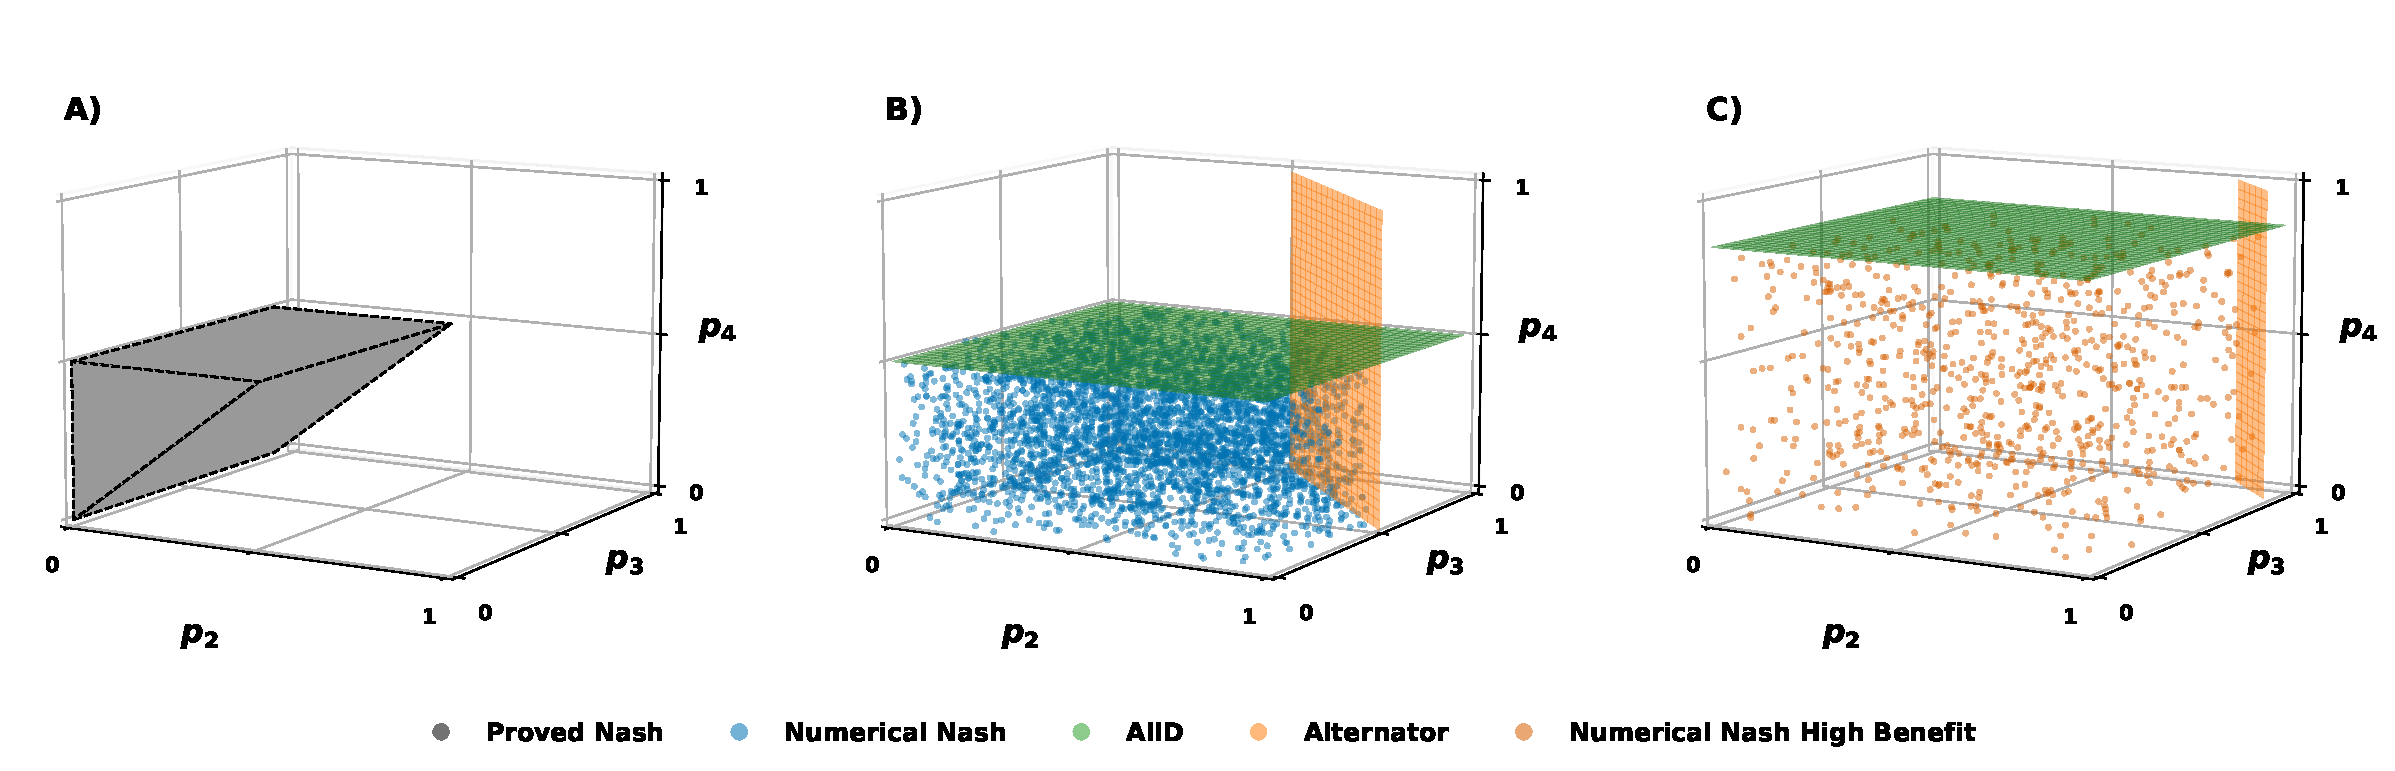
\includegraphics[width=\textwidth]{static/two_bit_reactive_numerical_results.pdf}
     \caption{\textbf{Nash results for two-bit strategies.}
     \textbf{A) Proved Nash.} We have shown that if a two-bit reactive
     strategy is within this space, thus satisfies conditions
     (\ref{eq:nash_conditions}), then it is good Nash. \textbf{B) Numerical nash
     results.} The results from
     Algorithm~\ref{algorithm:numerical_nash}. We evaluated \(10 ^ 4\) points in
     the space. The numerical results have shown that there are two pure
     strategies that constrain the Nash space; these are AllD and Alternator.
     The equations for the planes are obtained by solving
     \(\pi(\mathbf{q}, \mathbf{\hat{p}}) = (b\!-\!c)\). The equations are
     \(\hat{p}_4 = 1 - \frac{c}{b} \text{ and }  \hat{p}_3 = 1 + \frac{b\!-\!c}{c} - \hat{p}_2\).
      Parameters: \(c=1, b=2\). \textbf{C) Numerical Nash for high benefit.} We repeat
     Algorithm~\ref{algorithm:numerical_nash} for a higher value of benefit
     (\(b=7\)) for \(10 ^ 3\) random points. We can see that the strategies AllD
     and Alternator still constrain the space of possible Nash. Note that we do
     not plot \(\hat{p}_1\) for any of the above plots, since \(\hat{p}_1=1\).}\label{fig:two_bit_reactive_nash_results}
\end{figure}

\nikoleta{The Python script to run the numerical evalution is
`src/numerical\_equilibria\_n\_bit.py'. The analysis of the results and the code
for the plot are in the notebooks `3.2. A numerical evaluation of good
strategies for n = 2 [Plots]' and `3.2. A numerical evaluation of good
strategies for n = 2'.}

\subsection{A numerical evaluation of good (\(n=2\)) reactive strategies for the prisoner's dilemma}\label{section:good_strategies_numerically_pd}

The payoff matrix~(\ref{eq:donation_payoffs}) is a special case of the
prisoner's dilemma known as the donation game. In the general case the
prisoner's dilemma the payoffs of a player \(p\) are given by the following
payoff matrix,

\begin{equation}\label{eq:pd_payoffs}
  \begin{blockarray}{ccc}
      & \text{cooperate} & \text{defect} \\
      \begin{block}{c(cc)}
          \text{cooperate} & R & T \\
          \text{defect} & S & P \\
      \end{block}
  \end{blockarray}
\end{equation}

where \(R\) is the reward for mutual cooperation, \(T\) is the temptation to
defect, \(S\) is the payoff of the sucker and \(P\) is the punishment for mutual
defection. We have also carried out the numerical evaluation of Nash using the
payoff matrix~(\ref{eq:pd_payoffs}) with values \(R=0.6, T=1, S=0\) and
\(P=0.1\).

Since a two-bit reactive strategy \(\mathbf{\hat{p}} = (\hat{p}_{1},
\hat{p}_{2}, \hat{p}_{3}, \hat{p}_{4})\) can only be a Nash equilibrium if {\it
no} other strategy yields a larger payoff, in particular neither \text{AllD},
nor \text{Delayed Alternator}, nor N8898 strategy must yield a larger payoff, where AllD\(=(0,
0, 0, 0, 0, 0, 0, 0, 0, 0, 0, 0, 0, 0, 0, 0)\), Delayed Alternator\(=(0, 0, 0,
0, 0, 0, 0, 0, 1, 1, 1, 1, 1, 1, 1, 1)\) and N8898\(=(0, 0, 1, 0, 0, 0, 1, 0, 1,
1, 0, 0, 0, 0, 1, 0)\).

We conclude that an agreeable two-bit reactive strategy  \(\mathbf{\hat{p}} =
(\hat{p}_{1}, \hat{p}_{2}, \hat{p}_{3}, \hat{p}_{4})\) can only form a Nash
equilibrium if

\begin{align*}
\pi(\text{AllD}, \mathbf{\hat{p}}) \leq R & & \pi(\text{Delayed Alternator}, \mathbf{\hat{p}}) \leq R & & \pi(\text{N8898}, \mathbf{\hat{p}}) \leq R.
\end{align*}

Assuming without loss of generality that $T\!=\!1$ and $S\!=\!0$, these conditions are equivalent to

\begin{align}\label{Eq:NashConditionDonationGamePD}
  \hat{p}_4 \leq \frac{P}{P - 1} & & \hat{p}_3 + \hat{p}_4 \geq \frac{P \cdot (\hat{p}_2 - 1) + 4 \cdot R - \hat{p}_2 - 1}{R} &  &  \hat{p}_2 + \hat{p}_3 \leq 3 - \frac{1}{R}.
\end{align}

In fact, a further numerical analysis (Figure~\ref{fig:numerical_results_prisoners_dilemma}) suggests the following stronger result. 

\begin{conjecture}\label{conjecture:nash_from_numerical_results_pd}
For a general repeated prisoner's dilemma with payoffs $1=T>R>P>S=0$ and $2R>T\!+\!S=1$, an agreeable two-bit reactive strategy \(\mathbf{\hat{p}} = (\hat{p}_{1}, \hat{p}_{2}, \hat{p}_{3}, \hat{p}_{4})\) is of Nash type if and only if conditions \eqref{Eq:NashConditionDonationGamePD} hold.
\end{conjecture}

\begin{figure}[!htbp]
  \centering
  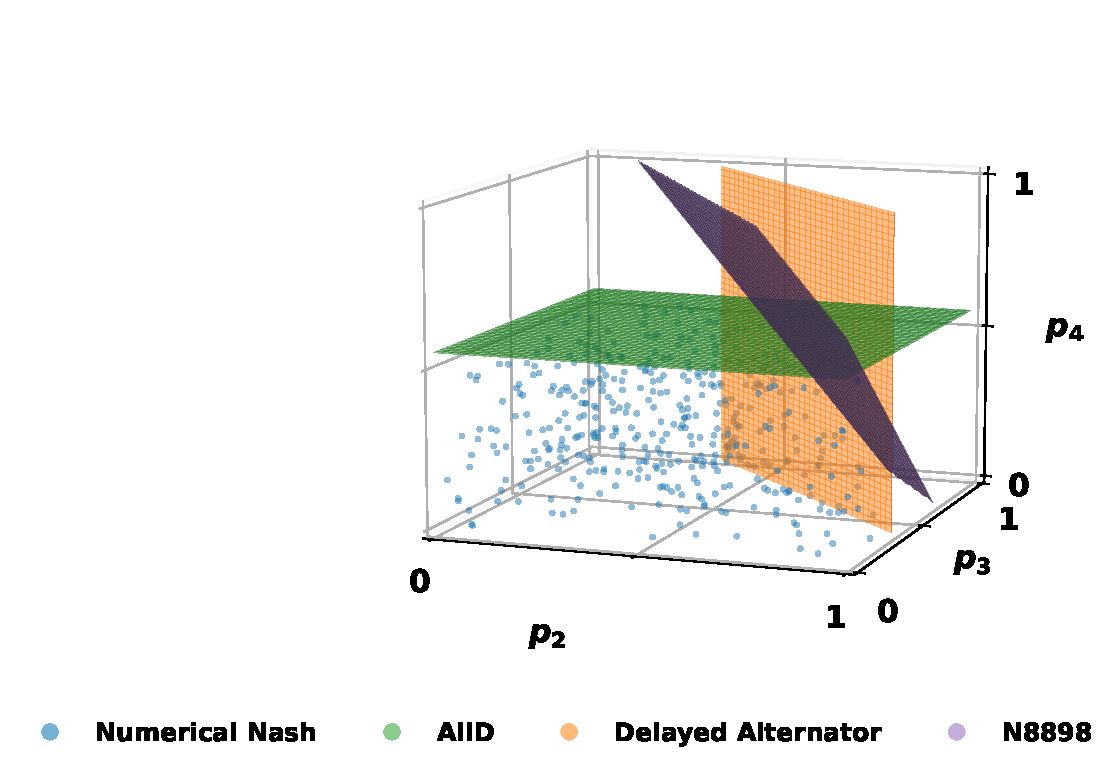
\includegraphics[width=.55\textwidth]{static/two_bit_reactive_numerical_results_prisoners_dilemma.pdf}
  \caption{\textbf{Nash results for two-bit strategies for the prisoner's dilemma.}
  We performed Algorithm~\ref{algorithm:numerical_nash} for \(10 ^ 3\) random
  points. Now the payoffs are given by matrix~(\ref{eq:pd_payoffs})
  with \(R=0.6, T=1, S=0\) and \(P=0.1\). There are several triples of
  strategies that can constrain the Nash space, such a triple is AllD, Delayed
  Alternator and N8898. To derive this triple we followed the same approach as
  in section~\ref{section:good_strategies_numerically}.}
  \label{fig:numerical_results_prisoners_dilemma}
\end{figure}

\nikoleta{The Python script to run the numerical evalution is
`src/numerical\_equilibria\_n\_bit.py'. The analysis of the results and the code
for the plot are in the notebook `3.3 A numerical evaluation of good strategies
(n = 2) for the prisoner's dilemma'. There is mathematica file
`src/mathematica/prisoners\_dilemma', to get the conditions for Nash based on
the Akin approach.}

\subsection{A numerical evaluation of good memory-two strategies}\label{section:good_strategies_numerically_mem_two}

We can repeat the same process for the case of memory-two strategies for the
donation game. We evaluated \(10^3\) random points for the parameter values \(b=2\)
and \(c=1\). The numerical results show that in the case of memory-two strategies,
Theorem~\ref{theorem:memory_two_nash_and_good}, is also sufficient but not
necessary. We hypothesise that even though our methodology can be applied to
greater memory sizes, the space that the derived conditions will explain will
reflect a smaller and smaller portion of the feasible Nash space.

We have also tried to obtain the smallest possible subset of strategies that can
constrain the space of Nash, similar to the donation game (AllD and Alternator)
and the prisoner's dilemma (AllD, Delayed Alternator and N8898) for two-bit
reactive strategies. We can show that a pair of such strategies does not exist.
Excluding AllD, there are a total of 35,766 strategies that their sets'
combination could potentially  be the smallest sub-collection necessary to
explain Nash. However, this is a problem that we can not solve explicitly.
Instead we have to consider an approximate solution using a greedy algorithm.

Initially, we remove all the elements in the elements from the universe that are
covered by AllD. The algorithm takes an input a starting strategy (and
subsequently its set), and thereafter at each stage it chooses the strategy that
contains the largest number of uncovered elements. In the case that two or more
strategies have contain the same number of uncovered elements, the algorithm
randomly picks one. We run the algorithm for 3467 initial conditions, and for
each we repeat the process 20 times. The initial conditions were chosen based on
the largest number of uncovered elements. For each run we record the output
subset and its size. The results are given by
Table~\ref{table:greedy_algorithm}. Note that the minimum subset size includes
AllD that we initially excluded.

\begin{table}[htbp]
  \centering
  \resizebox{.45\linewidth}{!}{%
   \begin{tabular}{l c c}
  \toprule
   & Min subset size & Num. of times solution was reached \\
  \midrule
  & 15 & 3899 \\
  & 14 & 19856 \\
  & 13 & 28385 \\
  & 12 & 14876 \\
  & 11 & 1964 \\
   \bottomrule
\end{tabular}}
\caption{\textbf{Results of greedy algorithm.} The greedy algorithm was used to
find the smallest possible subset of pure memory-two strategies that can
constrain the space of Nash in the case of memory-two strategies. Based on the
approximate solution, the smallest subset is of size
11.}\label{table:greedy_algorithm}
\end{table}

\nikoleta{The python script to run the greedy algorithm is `src/set\_cover.py',
and the analysis of the results is in the
notebook `nbs/3.4 A numerical evaluation of good memory-two strategies'.
The notebook also contains the analysis of the numerical results for this case.
The script for the numerical Nash is `src/numerical\_equilibria\_memory\_n.py'.}

\subsection{Pure \(n-\)bit Reactive Strategies with Errors}\label{section:pure_strategies}

The aim of the section is to explore if there are pure reactive strategies that
are evolutionary stable. In this section we consider the donation game with
noise. Noise is a given probability \(\epsilon\) that a player's action is
flipped, such that if a player intends to cooperate the defect with a
probability \(\epsilon\).

The work of~\citep{hilbe:PNAS:2017} introduced a method that can identify all
(strict) Nash equilibria among a finite set of strategies, and for which
parameter values the respective strategy is stable (i.e., which benefit-to-cost
ratio b/c is required in the donation game). We refer to this method as the
Martinez-Vaquero method, and a description of the method can be found in
Appendix~\ref{section:matrinez_vaquero_method}. Note that one of the assumptions
of the method is that \(\epsilon \neq 0\).

We apply the Martinez-Vaquero method and identify all the pure strict Nash
equilibria in the case where players are allowed to choose from the sets of (i)
one-bit (ii) two-bits and (ii) three-bits reactive strategies for a small error
rate of \(\epsilon=0.01\). The results are given in
Table~\ref{table:pure_nash_results}.


\begin{table}[htbp]
  \centering
  \resizebox{\linewidth}{!}{%
   \begin{tabular}{c c c c c}
  \toprule
   & Strategy & \(\rho\) (self coop. rate) & Min. \(\frac{b}{c}\) ratio & Max. \(\frac{b}{c}\) ratio \\
  \midrule
   \multirow{ 1}{*}{One-bit reactive} & \(p_1 = 0, p_2 = 0\) & 0 & 0 & 0\\
   \midrule
   \multirow{ 2}{*}{Two-bit reactive} & \(p_1 = 0, p_2 = 0, p_3=0, p_4=0\) & 0.0 & None & None\\
   & \(p_1 = 0, p_2 = 1, p_3=0, p_4=0\) & 0.255 & 1.04 & None \\
   & \(p_1 = 0, p_2 = 0, p_3=1, p_4=0\) & 0.255 & 1.04 & None \\
   \midrule
   \multirow{ 3}{*}{Three-bit reactive} &  \(p_1 = 0, p_2 = 0, p_3=0, p_4=0, p_5=0, p_6=0, p_7=0, p_8=0\) & 0.0 & None & None\\
   & \(p_1 = 0, p_2 = 0, p_3=0, p_4=0, p_5=0, p_6=1, p_7=0, p_8=0\) & 0.182 & 1.0590 & 1.0592 \\
   & \(p_1 = 0, p_2 = 0, p_3=1, p_4=0, p_5=0, p_6=0, p_7=1, p_8=0\) & 0.255 & 1.041 & 1.042 \\
   \bottomrule
\end{tabular}}
\caption{\textbf{Pure one, two and three bit(s) reactive strategies.} The
Martinez-Vaquero method allows us to numerically evaluate if pure strategies are evolutionary stable given that
errors can occur. We performed the algorithm for a small percentage of error
\(\epsilon=0.01\). The table shows all pure reactive strategies that are strict Nash,
the \(\frac{b}{c}\) ratio for which they are Nash and for each strategy the cooperating rate
against itself. Overall, there are only a few reactive strategies that
are Nash. In the case of two-bit reactive strategies there are only three. In~\cite{hilbe:PNAS:2017}
The method is applied to memory-two strategies and they show that there are 27
strategies that are Nash. This includes cooperative strategies (\(\rho=1\)).
In the case of reactive strategies, regardless of the memory size there are no
cooperative strategies that sustain an equilibrium. For all strategies in this table
\(\rho \leq 0.255\). 0.255 corresponds to a quarter of cooperation.
AllD is the only pure strategy that is stable regardless of the memory size. In the
case of two-bit strategies the only other strategies that are stable are
strategies that defect following a defection of the co-player. In the case of the
three-bit reactive strategies only 3/64 strategies that can
sustain an equilibrium, and for very few values of  \(\frac{b}{c}\) ratio. Thus, these strategies
are not too robust in the sense that a small change in the payoff ratio
results in them not being stable.}\label{table:pure_nash_results}
\end{table}

In the case of reactive strategies there are no cooperative pure
strategies that are evolutionary stable in the presence of noise. This could
indicate that in the case of reactive strategies, where memory is even more
limited compared to memory-\(n\) strategies, stochasticity can be important.

\nikoleta{The Matlab code for running the simulations is in the folder
`src/matlab\_code', and the analysis of the results was done in the
notebook `nbs/3.5. Pure Nash with Noise'.}

\subsection{Evolutionary Dynamics}\label{section:evolutionary_simulations}

In this section, we explore whether cooperative equilibria evolve. Moreover,
previous studies (\citep{hilbe:PNAS:2017}) have shown that in the case of
memory-\(n\) strategies for intermediate b/c ratios, cooperation should more
readily evolve among strategies with more memory. Here we also test if this
result holds for reactive strategies.

To examine the evolutionary properties on \(n-\)bit reactive strategies, we
perform an evolutionary study based on the framework of Imhof and
Nowak~\citep{imhof:royal:2010}. The framework considers a population of size
\(N\) where initially all members are of the same strategy. In our case the
initial population consists of unconditional defectors. In each elementary time
step, one individual switches to a new mutant strategy. The mutant strategy is
generated by randomly drawing cooperation probabilities from the unit interval
\([0,1]\). If the mutant strategy yields a payoff of \(\pi_{M}(k)\), where \(k\)
is the number of mutants in the population, and if residents get a payoff of
\(\pi_{R}(k)\), then the fixation probability \(\phi_{M}\) of the mutant
strategy can be calculated explicitly,

\begin{equation}\label{eq:fixation_probability}
  \phi_{M} = \left(1 + \sum_{i=1}^{N - 1} \prod_{j=1}^{i} \text{exp} (- \beta (\pi_{M}(j) - \pi_{R}(i))) \right)^{-1}
\end{equation}

The parameter \(\beta \geq 0\) is called the strength of selection, and it
measures the importance of the relative payoff advantages for the
evolutionary success of a strategy. For small values of \(\beta\), \(\beta
\approx 0\), payoffs become irrelevant, and a strategy's fixation probability
approaches \(\phi_{M} \approx 1 / N\). The larger the value of \(\beta\), the
more strongly the evolutionary process favours the fixation of strategies that
yield high payoffs.

Depending on the fixation probability \(\phi_{M}\) the mutant either fixes
(becomes the new resident) or goes extinct. Regardless, in the elementary time
step another mutant strategy is introduced to the  population. We iterate this
elementary population updating process for a large number of mutant strategies
and we record the resident strategies at each time step.

To study the effects of memory size we perform this evolutionary process when
the population draws strategies from the sets of (i) one-bit (ii) two-bits and
(ii) three-bits reactive strategies. We initially test the evolving cooperation
rates for different selection strengths, Figure~\ref{fig:three_graphs}. To this end, we ran simulations for
different b/c ratios. As expected, higher b/c values lead to more cooperation in
all three spaces, and regardless of \(\beta\)'s value. However, the more memory
a strategy has it requires a lower benefit-to-cost ratio to achieve substantial
cooperation. This verifies that the results of~\citep{hilbe:PNAS:2017} also
hold for reactive strategies.

We then explore the type of strategies that evolve for each set of reactive
strategies, Figure~\ref{fig:three_graphs}. In all cases, the most abundant
strategy achieves a high cooperation rate against itself. Notice that all most
abundant strategies are the harsher when the co-player defects for the first
time after a series of \(n - 1\) cooperations. We can observe that in both the
case of the two-bits and three-bits, the strategies are more forgiving towards
two defections.

\begin{figure}[htbp]
  \centering
  \begin{subfigure}{0.85\textwidth}
      \centering
      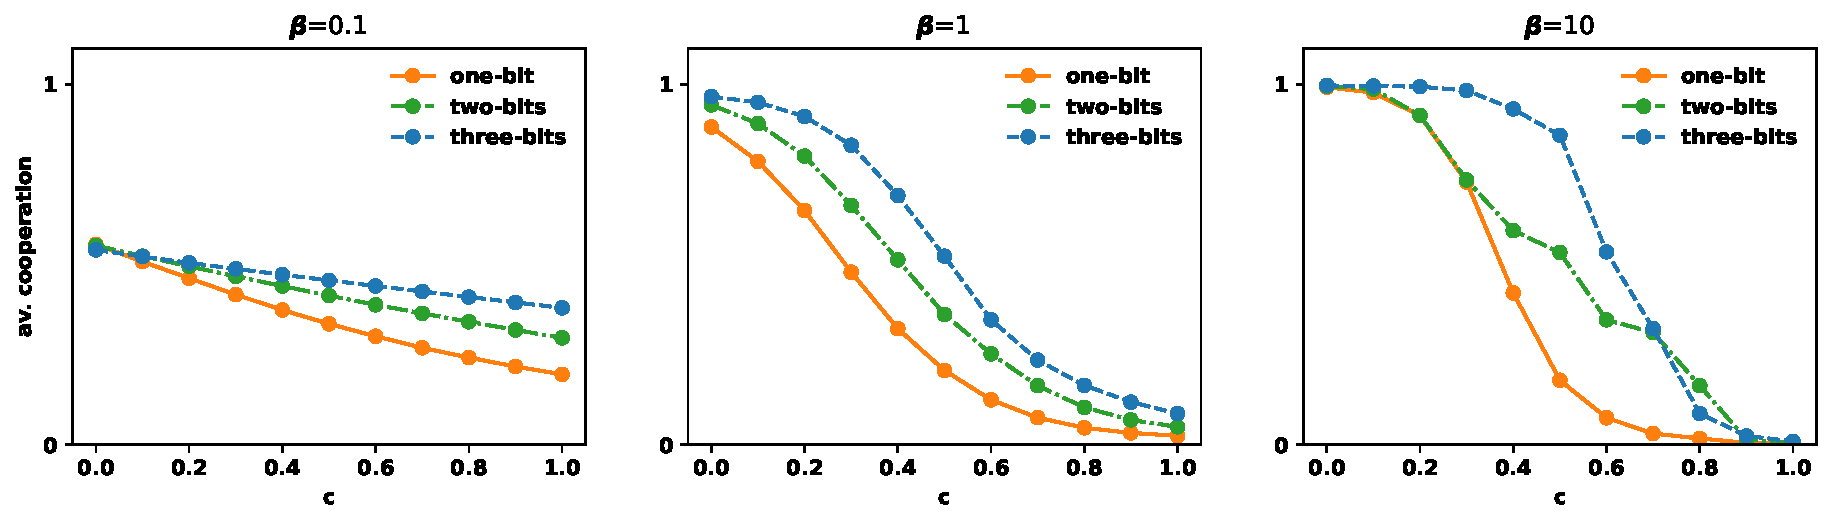
\includegraphics[width=\textwidth]{static/average_cooperation_over_c_with_diff_selection_strength.pdf}
  \end{subfigure}
  \hfill
  \begin{subfigure}{0.85\textwidth}
      \centering
      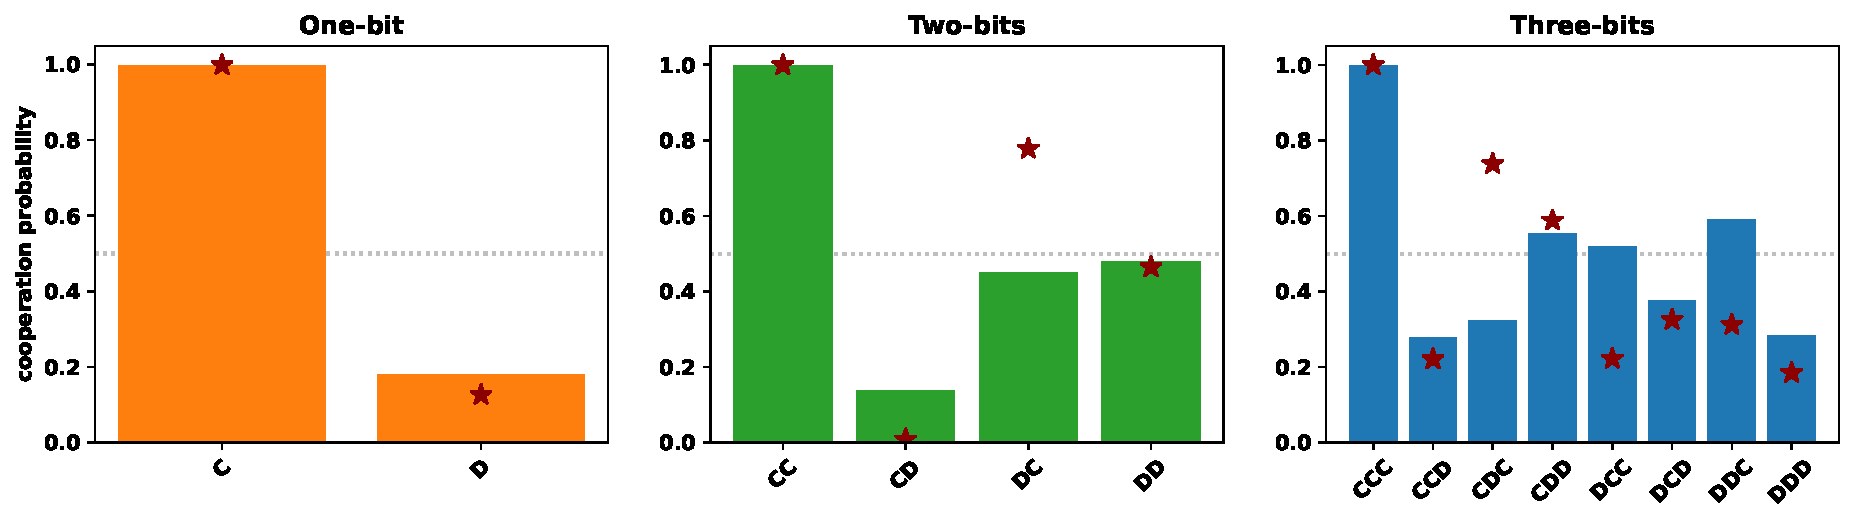
\includegraphics[width=\textwidth]{static/evolution_results_barplots.pdf}
  \end{subfigure}
  \hfill
  \begin{subfigure}{0.85\textwidth}
      \centering
      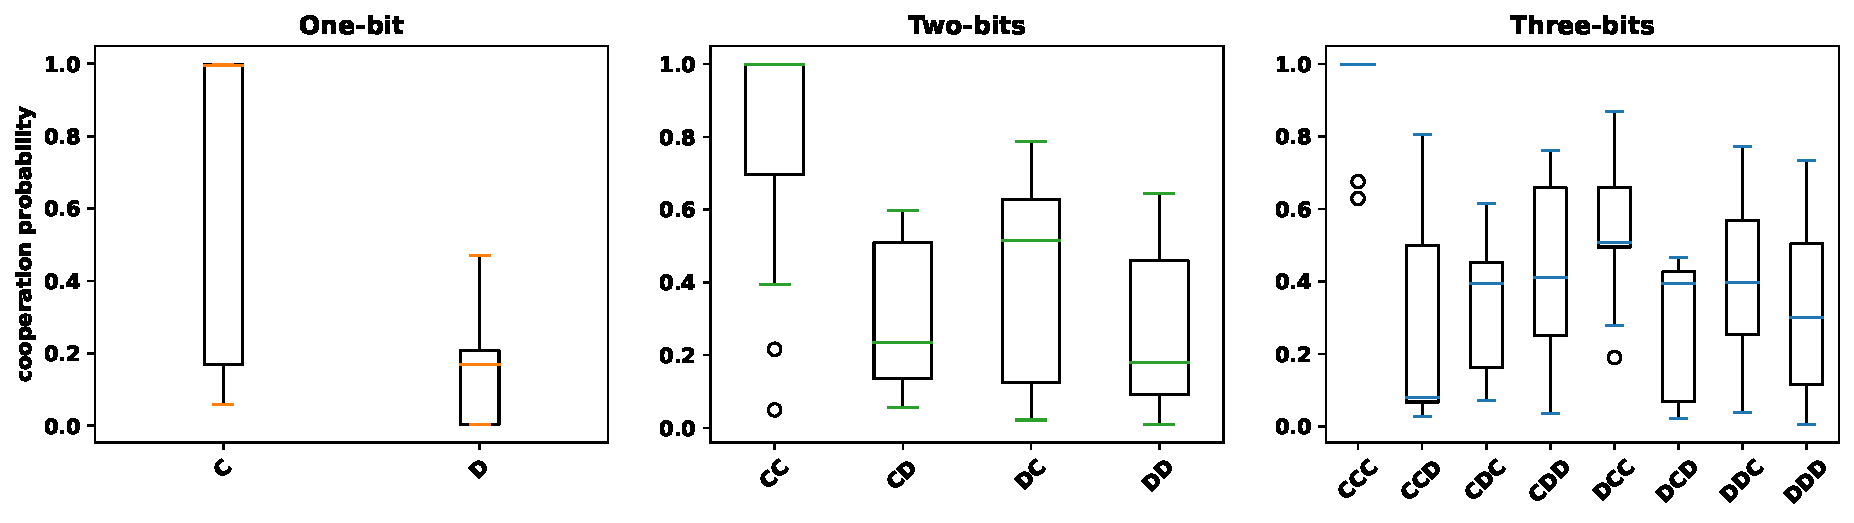
\includegraphics[width=\textwidth]{static/evolution_results_boxplots.pdf}
  \end{subfigure}
  \caption{\textbf{Comparing the evolving cooperation rates and the most
  abundant strategies  one-bit, two-bits, and three-bits strategies.}
  \textbf{A.} the evolving cooperation rates for different selection strengths.
  To assess the impact of memory on the evolution of cooperation, we ran
  simulations based on Imhof and Nowak for different benefit-to-cost ratios and
  different selection strengths. The average cooperation is calculated by
  considering the cooperation rate within the resident population. For a single
  run of the evolutionary process, we record the cooperating probabilities of
  the resident at each elementary time step. For each resident we estimate the
  cooperation rate between two resident strategies, and we take the average of
  that. 
  \textbf{B and C.} We ran 10 independent simulations for each set of strategies
  and recorded the most abundant strategy for each run. The abundant strategy is
  the resident that was fixed for the most time steps. For the simulations we
  used \(b=3 \text{ and } c=1\). The colored bars show the average values of
  cooperation probabilities of the most abundant strategies. The stars show the
  cooperation probabilities of the most abundant strategy for each set. The
  boxplots illustrate the distributions of cooperation probabilities for the ten
  runs.
  Parameters: \(N=100\), \(\beta=1\). Each simulation was run for \(10 ^ {5}\)
  mutant strategies except for the simulations where \(\beta=10\). These we
  run for \(2 \cdot 10 ^ {5}\).}\label{fig:three_graphs}
\end{figure}

\nikoleta{The Matlab code for running the simulations is in the folder
`src/matlab\_code', and the analysis of the results was done in the
notebook `nbs/3.6. Evolutionary Simulations'.}

\newpage

\section{Conclusion}

In this work we have studied the space of \(n-\)bit reactive strategies. This space
was originally explored by the work of~\citep{nowak:AAM:1990}. The reactive
space contains many well known strategies from the literature, such as Grudger,
Tif For Tat and Generous Tit For Tat. However, note that these are reactive
strategies of memory size one. We referred to these as one-bit reactive
strategies. Here we aimed to explore higher memory reactive strategies, and even
though this has been done previously for memory\(-n\) strategies, many questions
still remain open in the case of reactive ones.

In section~\ref{section:good_nash_strategies} we analytically explored two-bit
reactive strategies. We built on the work of~\citep{akin:EGADS:2016} and proved
that there is a set of stochastic two-bit strategies that can sustain
cooperative Nash equilibria. More specifically, we derived four conditions that
must be true for a strategy in order to be a good Nash. In
section~\ref{section:good_strategies_numerically}, we aimed to verify our
results using numerical simulations. Though the conditions derived in
section~\ref{section:good_nash_strategies} are sufficient, they are not
necessary.

We also applied our methodology to the case of memory-two strategies, and showed
very similar results. Though there is a subset of memory-two strategies that we
can prove are Nash, the numerical simulations suggest that the conditions are
only sufficient~\ref{section:good_strategies_numerically_mem_two}.

In~\citep{akin:EGADS:2016} it is also proven that for a strategy to be Nash it
is enough to check that the strategy is Nash against two pure memory-one
co-players. From the numerical simulations we have obtained a similar result for
the case of two-bit reactive
strategies~\ref{section:good_strategies_numerically}
and~\ref{section:good_strategies_numerically_pd}.

In the case of pure reactive strategies we showed that when there is a
vanishingly small probability of error, no cooperative Nash is evolutionary
stable~\ref{section:pure_strategies}. We
built on the work of~\citep{hilbe:PNAS:2017} where they numerically showed that
memory-\(n\) cooperative Nash are stable. Thus, we can see that constraining
the information a strategy receives to only the co-players moves makes it harder
for cooperation.

In the last section~\ref{section:evolutionary_simulations}, we explored the
space of reactive strategies with evolutionary simulations. Though cooperative
Nash can be obtained, here we asked the question: can they also evolve? In all
the cases we have presented, high levels of cooperation can be achieved but
larger memory allows for cooperation to emerge faster.


\appendix

\section{The Martinez-Vaquero Method}\label{section:matrinez_vaquero_method}

Let \(p\) and \(q\) play as \(\mathbf{p}_{\epsilon}\) and
\(\mathbf{q}_{\epsilon}\) from a given set of strategies in a noisy environment
with \(\epsilon > 0\) where \(\mathbf{p}_{\epsilon} = \epsilon(1 - \mathbf{p}) +
(1 - \epsilon)\mathbf{p} \). Given the two strategies we numerically compute
the three following measures:


\begin{itemize}
  \item The fraction of rounds \(\rho\) in which player \(p\) cooperates against itself.
  \item The fraction of rounds \(\tilde{\rho}_p\) in which player \(p\) cooperates against \(q\).
  \item The fraction of rounds \(\tilde{\rho}_q\) in which player \(q\) cooperates against \(p\).
\end{itemize}

Given these measures the payoffs for \(p\) against itself can given by,

\[\pi (\mathbf{p}, \mathbf{p}) = b \cdot \rho - c\cdot\rho,\]

and the payoffs for \(q\) against \(p\) by,

\[\pi(\mathbf{q}, \mathbf{p}) = b \cdot \tilde{\rho}_p - c\cdot\tilde{\rho}_q.\]

For \(\mathbf{p}_{\epsilon}\) to be a Nash equilibrium, it needs to be the case that \(\pi (\mathbf{p}, \mathbf{p}) \geq
\pi(\mathbf{q}, \mathbf{p})\), that is

\begin{equation}\label{eq:nash_vaquero}
  b \cdot x_{\mathbf{p}, \mathbf{q}} \geq c \cdot y_{\mathbf{q}, \mathbf{p}}
\end{equation}

where \(x_{\mathbf{p}, \mathbf{q}} = \rho - \tilde{\rho_p}\) and  \(y_{\mathbf{q}, \mathbf{p}} = \rho - \tilde{\rho_q}\).
For \(p\) to be a strict Nash equilibrium, the inequality (\ref{eq:nash_vaquero}) needs
to be strict. Since \(b > c > 0\), there are four possible cases

\begin{enumerate}
  \item \(x_{\mathbf{p}, \mathbf{q}} > 0 \) and \(y_{\mathbf{q}, \mathbf{p}} > 0\). In that case, \(\mathbf{p}\) is stable
  against \(\mathbf{q}\) if \(b/c \geq y_{\mathbf{q}, \mathbf{p}}/x_{\mathbf{p}, \mathbf{q}}\) (and it is strictly stable if the inequality is
  strict).
  \item \(x_{\mathbf{p}, \mathbf{q}} > 0 \) and \(y_{\mathbf{q}, \mathbf{p}} \leq 0\). In that case, \(\mathbf{p}\) is stable
  against \(\mathbf{q}\) if \(b/c \leq y_{\mathbf{q}, \mathbf{p}}/x_{\mathbf{p}, \mathbf{q}}\) (and it is strictly stable if the inequality is
  strict).
  \item \(x_{\mathbf{p}, \mathbf{q}} \leq 0 \) and \(y_{\mathbf{q}, \mathbf{p}} > 0\). In that case,
  \(\mathbf{p}\) is never stable against \(\mathbf{q}\), for no b/c ratio.
  \item  \(x_{\mathbf{p}, \mathbf{q}} \geq 0 \) and \(y_{\mathbf{q}, \mathbf{p}} \leq 0\). In that case, \(\mathbf{p}\) is stable against \(\mathbf{q}\) for any b/c ratio.
\end{enumerate}

Given the above we can define four sets:

\begin{align}
  Q_1(p) & = \{q \; | \; x_{\mathbf{p}, \mathbf{q}} > 0 \text{ and } y_{\mathbf{q}, \mathbf{p}} > 0 \}, \\
  Q_2(p) & = \{q \; | \; x_{\mathbf{p}, \mathbf{q}} < 0 \text{ and } y_{\mathbf{q}, \mathbf{p}} \leq 0 \}, \\
  Q_3(p) & = \{q \; | \; x_{\mathbf{p}, \mathbf{q}} \leq 0 \text{ and } y_{\mathbf{q}, \mathbf{p}} > 0\}, \\
  Q_4(p) & = \{q \; | \; x_{\mathbf{p}, \mathbf{q}} = 0  \text{ and } y_{\mathbf{q}, \mathbf{p}} = 0 \}, \\
\end{align}

It follows that \(\mathbf{p}\) is a Nash equilibrium if and only if \(Q_3(p) = \emptyset\)
and

\begin{equation}\label{eq:nash_vaquero_inequalities}
  \text{max}\{ \frac{y_{\mathbf{q}, \mathbf{p}}}{x_{\mathbf{p}, \mathbf{q}}} | q \in Q_1(p) \} \leq b / c  \leq \text{min}\{\frac{y_{\mathbf{q}, \mathbf{p}}}{x_{\mathbf{p}, \mathbf{q}}} | q \in Q_2(p) \}.
\end{equation}

\(\mathbf{p}\) is a strict Nash equilibrium if the inequalities in
(\ref{eq:nash_vaquero_inequalities}) are strict, \(Q_3(p) = \emptyset\) and
\(Q_4(p) = \emptyset\).

\section{Anti Press and Dyson}

The work of~\citep{press:PNAS:2012}, which is the work that introduced
zero determinant set of strategies, proved a further interesting result which
states the following:

\begin{theorem}[Iterated Prisoner's Dilemma contains strategies that dominate any evolutionary opponent]
  Let \(p\) play a short memory strategy, and \(q\) play with longer memory of
  the past outcomes. In the perspective of the forgetful strategy \(p\), \(p\)'s
  score is exactly the same as if \(q\) had played a certain shorter-memory
  strategy.
\end{theorem}

Thus, for a given memory-one strategy that interacts with a memory-two strategy,
the forgetful strategy will always be able to find a memory-one representation
for the memory-two co-player, such that its score remains the same.

Note that in sections~\ref{section:good_strategies_numerically}-
\ref{section:good_strategies_numerically_pd} when we explore whether a random
two-bit reactive strategy is Nash we check against all pure memory-two
strategies, not pure two-bit reactive strategies. In fact, it does not
suffice to check only pure two-bit reactive strategies.
That is because a \(n-\)bit reactive strategy can not guarantee that it will
find a reactive representation for a memory-\(n\) strategy. We refer to this
as the Anti Press and Dyson result.

For example, consider the case of \(n=1\). Let the reactive strategy
\(\mathbf{p} = (0, 0, 0, 0)\) and the memory-one co-player \(\mathbf{q} = (0, 0,
0, 1)\). \(p\) is a strategy that it always defects, and \(q\) cooperates
following a mutual defection, otherwise it defects. It is straightforward that
the pair gets stuck in a cycle of \(DD\) followed by \(DC\). Thus the stationary
distribution is \(\mathbf{v} = (0, 0, \frac{1}{2}, \frac{1}{2})\).

When the forgetful player \(p\) tries to estimate a strategy for its co-player
it will see that the co-player always cooperates given that it has defected in
the previous turn. Thus it estimates that the co-player must follow a strategy
\(\mathbf{q'} = (0, 1, 0, 1)\). However, between this new pair, \(\{CD\}\) is a
terminal set which is very different from the actual outcome. It's the
forgetfulness of \(p\) which forces \(q_2\) to be equal to 1.

\bibliography{bibliography.bib}

\end{document}